\section{A case for application-level multicast overlay}
\label{sec:motivation}

%\jc{Starting from Section 2, it would be paper outline.
%Please think each bullet point as a separate paragraph.}

%<<<<<<< HEAD
To provide a case for an
application-level multicast overlay network,
we first characterize the inter-DC multicast workload in
\company, a global-scale online service provider
(\Section\ref{subsec:motivation:multicast-traffic}).
We then show the potential of improving multicast performance
by leveraging disjoint application-level overlay paths available in geo-distributed DCs
(\Section\ref{subsec:motivation:case-for}).
Finally, we examine \company's existing solution to
inter-DC multicast and draw lessons from real-world
incidents (\Section\ref{subsec:motivation:baseline})
to inform the design of \name.
The findings are based on a dataset collected from \company's
inter-DC WANs over a duration of 7 days.
The dataset comprises of about 1265 data transfers
between over 30 geo-distributed DCs.
%\jc{what? i thought your results (table 1, fig 2, 4, 5) are
%based on much larger dataset?}


%=======
%We begin by motivating the need for an inter-DC multicast overlay.
%We first characterize the bulk-data multicast workload in \company
%a large-scale online service provider
%(\Section\ref{subsec:motivation:multicast-traffic}),
%as there is relatively little study on DC-level multicast
%traffic.
%We then show
%a substantial diversity in performance of application-level
%overlay paths, and thus make a case for an inter-DC multicast
%overlay that picks optimal overlay paths to optimize bulk-data
%multicast.
%(\Section\ref{subsec:motivation:case-for}).
%Finally, we study the operational experience of \company, a large
%online service provider, and draw important lessons from
%real-world incidents and statistics
%of the \company's existing multicast protocol
%(\Section\ref{subsec:motivation:baseline}).
%>>>>>>> 09029e454f71e5a5e01f13f554477705e665f4ec


\subsection{Characterizing inter-DC multicast workload}
\label{subsec:motivation:multicast-traffic}


\begin{table}[t!]
\begin{center}
\resizebox{3in}{!}{
%\begin{tabular}{p{2cm}<{\centering}|p{2cm}<{\centering}}
\begin{tabular}{| c | c|}
\hline
 \rowcolor[gray]{0.9}
\textbf{Type of application} & \textbf{Percent of multicast traffic} \\
\hline\hline
All applications & 91.13\%~\myfootnotemark\\
\hline
Blog posts & 91.0\% \\% 4648.92 vs 41372.56 in GB
\hline
Search indexing & 89.2\%\\% 16766.7 vs 138418.12
%\hline
%International & 98.15\%\\% 1297.7 vs 68699.97
\hline
Offline file sharing & 98.18\%\\% 2792.4 vs 150234.25
%\hline
%Scholar & 98.09\%\\% 451.22 vs 23134.21
\hline
Forum posts & 98.08\%\\% 964.62 vs 49327.01
\hline
Other DB sync-ups & 99.1\%\\% ?? vs ??
\hline
\end{tabular}
}
\end{center}
\tightcaption{Inter-DC multicast (replicating data from
one DC to many DCs) dominantes \company's inter-DC
traffic.}
\vspace{-0.2cm}
\label{table:rate}
\end{table}
\myfootnotetext{The overall multicast traffic share is estimated by that of the traffic goes through one randomly sampled DC, because we do not have access to information of all inter-DC traffic. But this number is consistent with what we observe on other DCs.}
%We randomly select one link from all inter-DC links whose traffic is monitored by different application types. As all these links carry the similar traffic, so the randomly selected one could exhibit good representatives.}

\mypara{Share of inter-DC multicast traffic}
%<<<<<<< HEAD
Table~\ref{table:rate} shows inter-DC multicast
(replicating data from one DC to multiple DCs) as
a fraction of inter-DC traffic.
We see that multicast traffic dominates \company's
overall inter-DC traffic (91.13\%), as well as
individual application types (89.2 to 99.1\%).
{\em The fact that inter-DC multicast traffic
amounting to a dominating share of inter-DC traffic
highlights the importance of optimizing its
performance.}
%=======
%First, we use \company's WAN to examine whether
%inter-DC multicast traffic (replicating data from
%one DC to multiple DCs)
%amounts to a substantial share of inter-DC traffic.
%Table~\ref{table:rate} shows multicast traffic as
%a fraction of inter-DC traffic across all applications as
%well as in some important application types individually.
%We see that multicast traffic dominantes the inter-DC traffic
%in \company, in terms of both overall traffic and
%several important types of application traffic,
%which highlights the importance of optimizing multicast
%traffic.
%>>>>>>> 09029e454f71e5a5e01f13f554477705e665f4ec
%To check the percentage of multicast traffic, we breakdown all \company's total traffic volume into non-multicast traffic and the multicast traffic of each application, and then calculate the share of multicast traffic. Table \ref{table:rate} shows that a considerably large fraction of traffic is multicast traffic, despite the application types. This result highlights the importance of bulk-data transmission optimization.


\begin{figure}[t]
        \centering
        \begin{subfigure}[b]{0.23\textwidth}
                \centering
                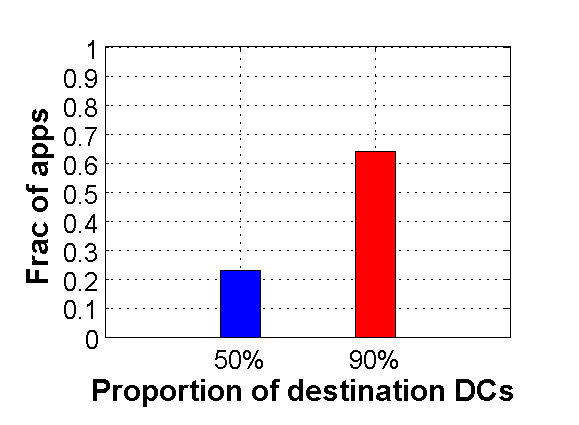
\includegraphics[width=\textwidth]{images/destinationDC.eps}%NeedMulticast.m
                \caption{Percent of multicast transfers destined to percent of DCs.}
                \label{fig:bulk:dest}
        \end{subfigure}
	\hspace{0.1cm}
        \begin{subfigure}[b]{0.23\textwidth}
                \centering
                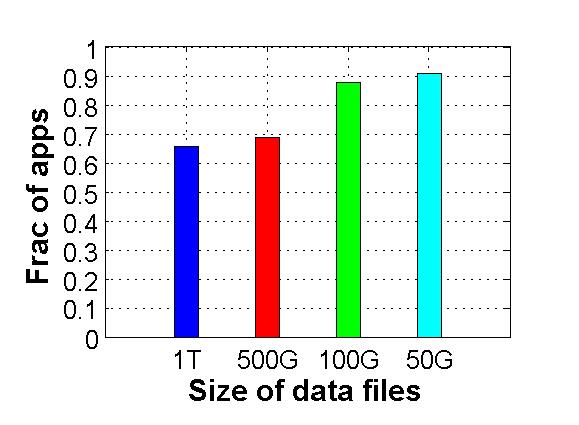
\includegraphics[width=\textwidth]{images/DataSize.eps}
                \caption{Percent of multicast transfers larger than certain threshold.}
                \label{fig:bulk:size}
        \end{subfigure}
        \vspace{-0.4cm}
        \tightcaption{Inter-DC multicasts (a) are destined to a significant
fraction of DCs and (b) have large data sizes.}
        \label{fig:bulk}
\vspace{-0.4cm}
\end{figure}

\vspace{0.1cm}
\noindent{\bf Where are inter-DC multicasts destined?}
%<<<<<<< HEAD
Next, we want to know if these transfers are destined to
a large fraction (or just a handful) of DCs, and whether
they have common destinations.
Figure~\ref{fig:bulk:dest} sketches the distribution of the
percentage of \company's DCs to which multicast
transfers are destined.
%=======
%In the premise that multicast traffic amount to a substantial
%fraction of traffic, we then examine whether these transfers
%are destined to just a handful of DCs.
%Figure~\ref{fig:bulk:dest} sketches the distribution of the
%percentage of DCs (in total, $\sim$ 30) to which multicast
%transfers are destined.
%>>>>>>> 09029e454f71e5a5e01f13f554477705e665f4ec
We can see that 90\% multicasts are destined
to over 60\% DCs, and 70\% are destined
to over 80\% DCs.
%<<<<<<< HEAD
Moreover, we found a great diversity in
source DCs and the sets of destination DCs (not shown here).
These observations suggest that {\em it is untenable
to pre-configure the data transfer for each possible multicast
request; instead, we need a scheme that automatically routes and
schedules data transfers for any given source and destination
DCs.}
%=======
%Moreover, we observed a great diversity (not shown)
%in terms of source DCs and the sets of destination DCs.
%Together, these observations suggest that it is undesirable to
%pre-configure the multicast overlay.
%>>>>>>> 09029e454f71e5a5e01f13f554477705e665f4ec

%In the premise that bulk data shares a large fraction of overall traffic, we check the number of destination DCs of the data. Fig. \ref{fig:bulk:dest} shows that there are over 60\% applications with bulk data multicast traffic are destined to at least 90\% DCs, and about 20\% applications with bulk data destined to over 50\% (but less than 90\%) DCs. These results show that a large fraction of the bulk data traffic is multicast to almost all DCs.

\mypara{Volumes of inter-DC multicast transfers}
Finally, Figure~\ref{fig:bulk:size} outlines the data size distribution of inter-DC multicast.
We see that over 60\% multicast data files are over 1TB
(and 90\% are over 50GB).
%<<<<<<< HEAD
Given that the total WAN bandwidth assigned to each multicast
is on the order of several Gb/s,
this suggests that the transfers are not transient but
typically last for a duration on the timescale of at least tens of
seconds instead. (The timescale is similar after optimization, see \Section\ref{sec:evaluation}).
Therefore, {\em any scheme that improves multicast traffic needs to
adapt to network dynamics.}
On the flip side, such temporal persistence
also indicates that {\em multicast traffic could tolerate certain delay
when adapting to changes in network conditions}, which inspires
\name's centralized design (\Section\ref{sec:overview}).
%=======
%The large data volumes suggest that the transfers are usually
%long-lived and thus we could improve multicast performance by
%routing data adaptively during a data transfer in response to
%dynamic network performance.
%>>>>>>> 09029e454f71e5a5e01f13f554477705e665f4ec


\vspace{0.1cm}
These observations motivate the need for a systematic approach
to optimizing inter-DC multicast.

%To further explore the characteristics of the multicast data files, we summarize the data size of these files and present the statistical results in Fig. \ref{fig:bulk:size}, which shows that nearly 70\% applications have a data file larger than 1TB and over 90\% of these multicast applications have data files larger than 50GB. Thus, focusing on optimizing bulk data multicast transmission is quite valuable to improve WAN conditions.

%\begin{itemize}
%
%\item Share of multicast traffic: use a bar chart to show the breakdown of all Baidu's total traffic volume into non-multicast traffic, and the multicast traffic of each application. {\em This should show a large fraction of traffic is multicast, and they are from many different applications.}
%
%\item A CDF of number of destination DCs. {\em This should show that most multicast traffic are destined to almost all DCs.}
%
%\item A CDF of size of multicast data files. {\em This should show that most multicast data are bulk data (not small data), and thus focusing on optimizing bulk data multicast is valuable.}
%
%\end{itemize}

\subsection{Potentials of inter-DC application-level overlay}
\label{subsec:motivation:case-for}

%\begin{figure}[t]
%\centering
%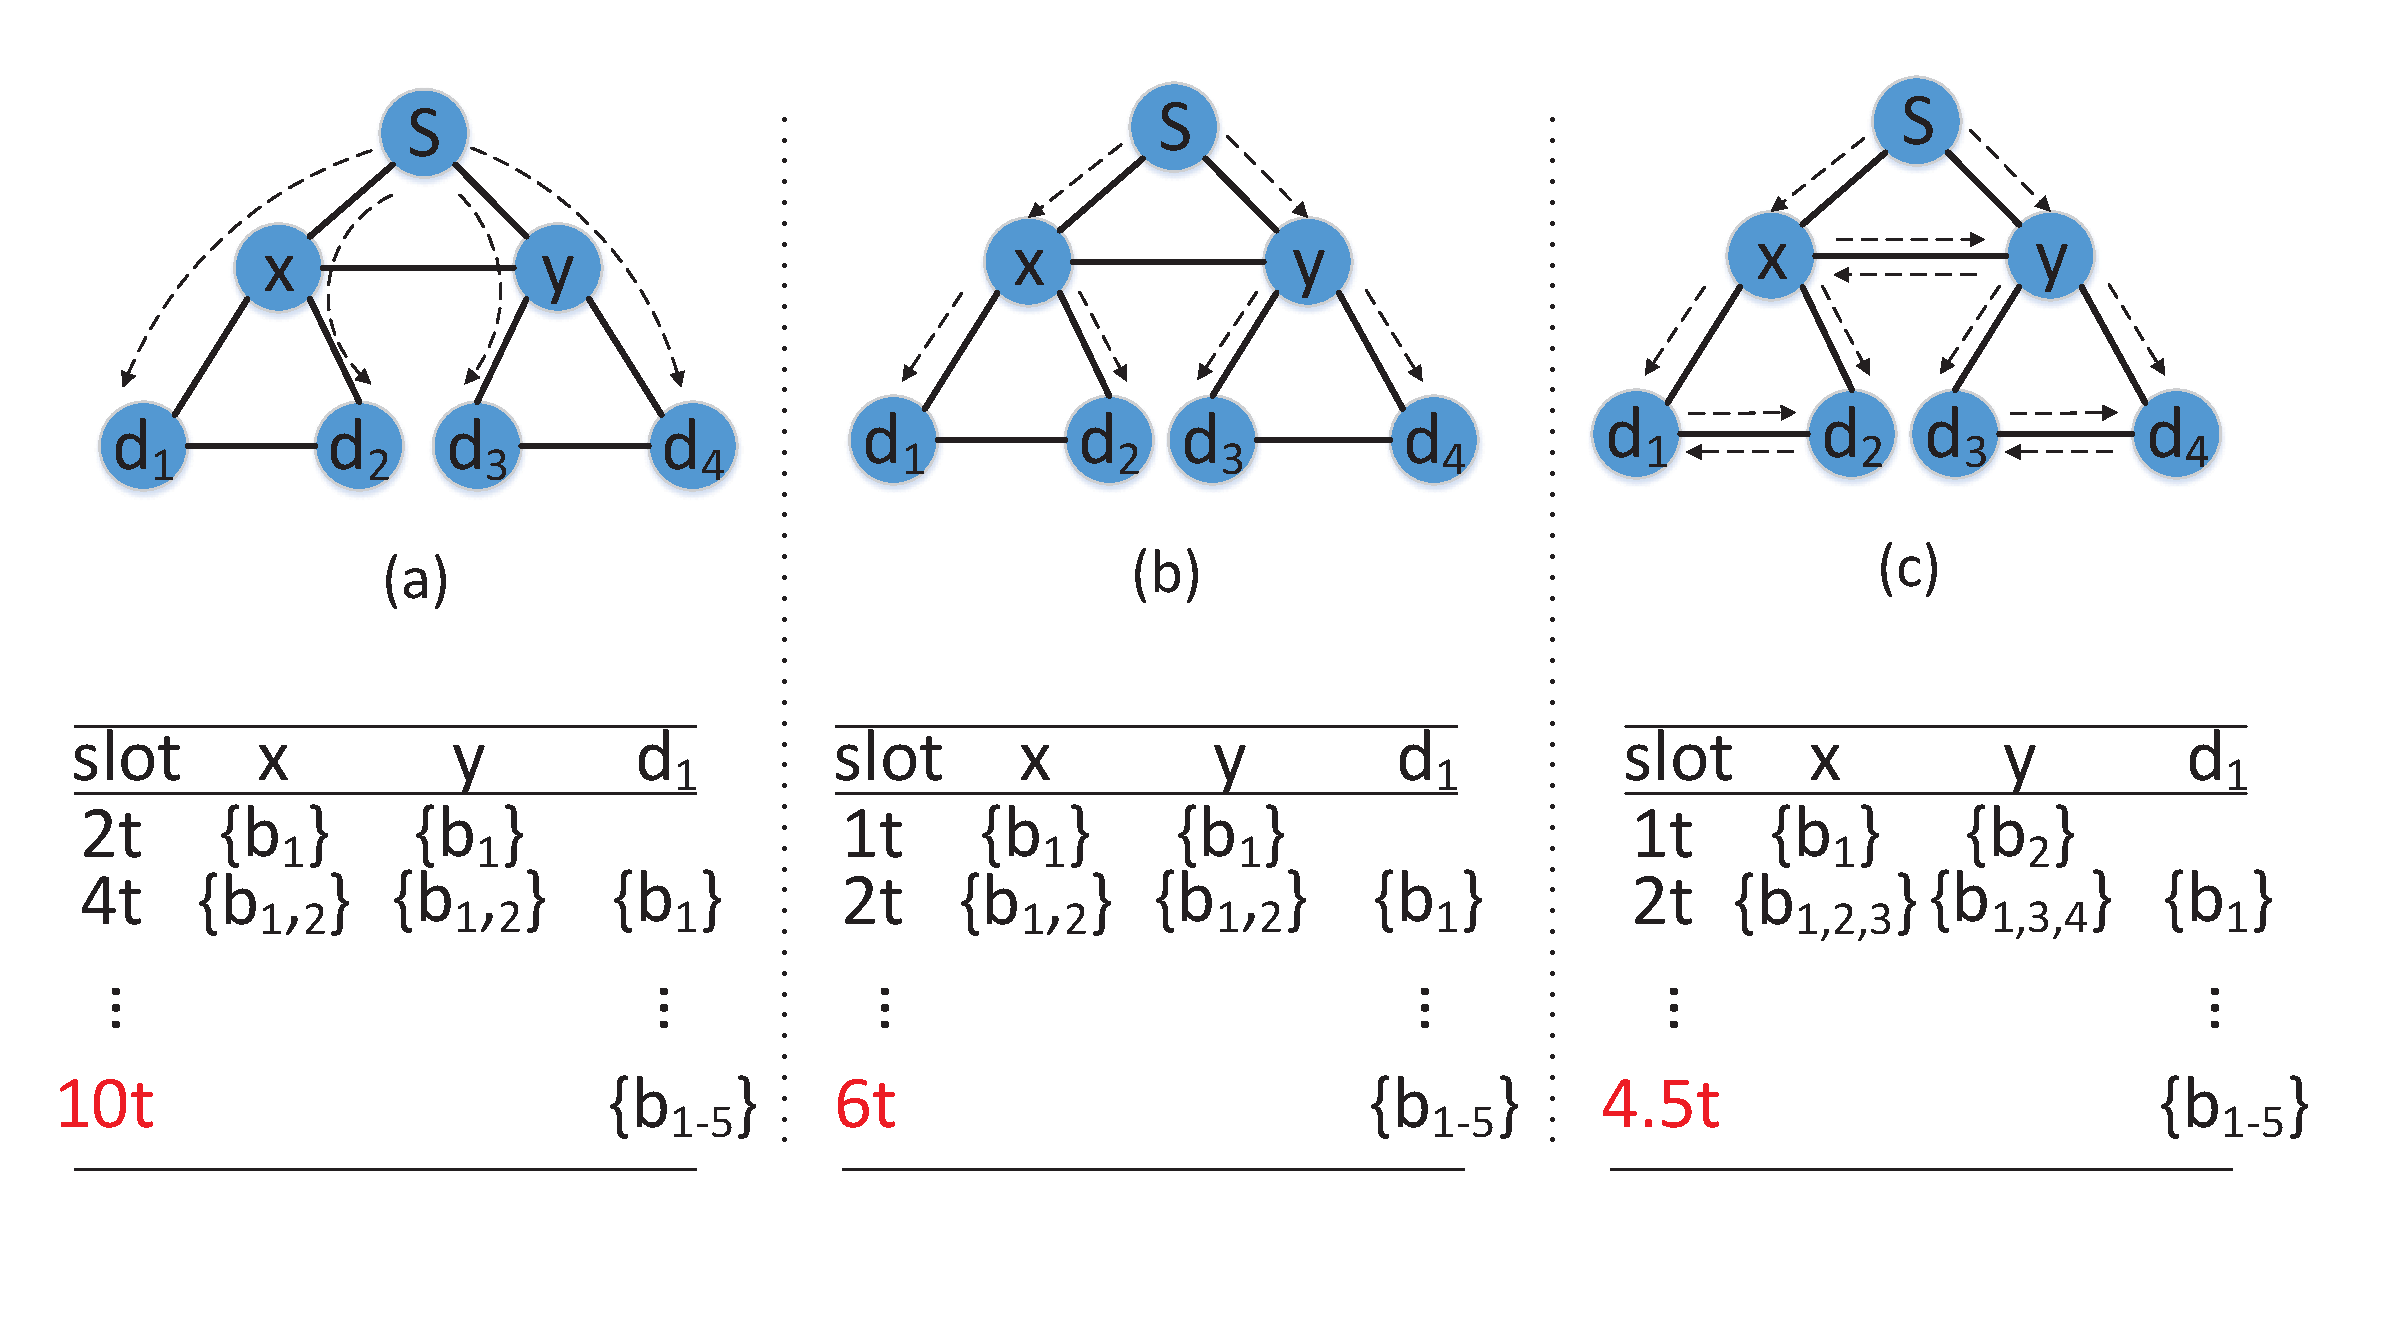
\includegraphics[width=80mm]{images/example.eps}
%\caption{A toy example showing the benefit from inter-DC multicast overlay.}
%\label{fig:case:example}
%\vspace{-0.4cm}
%\end{figure}

\begin{figure}[t]
\centering
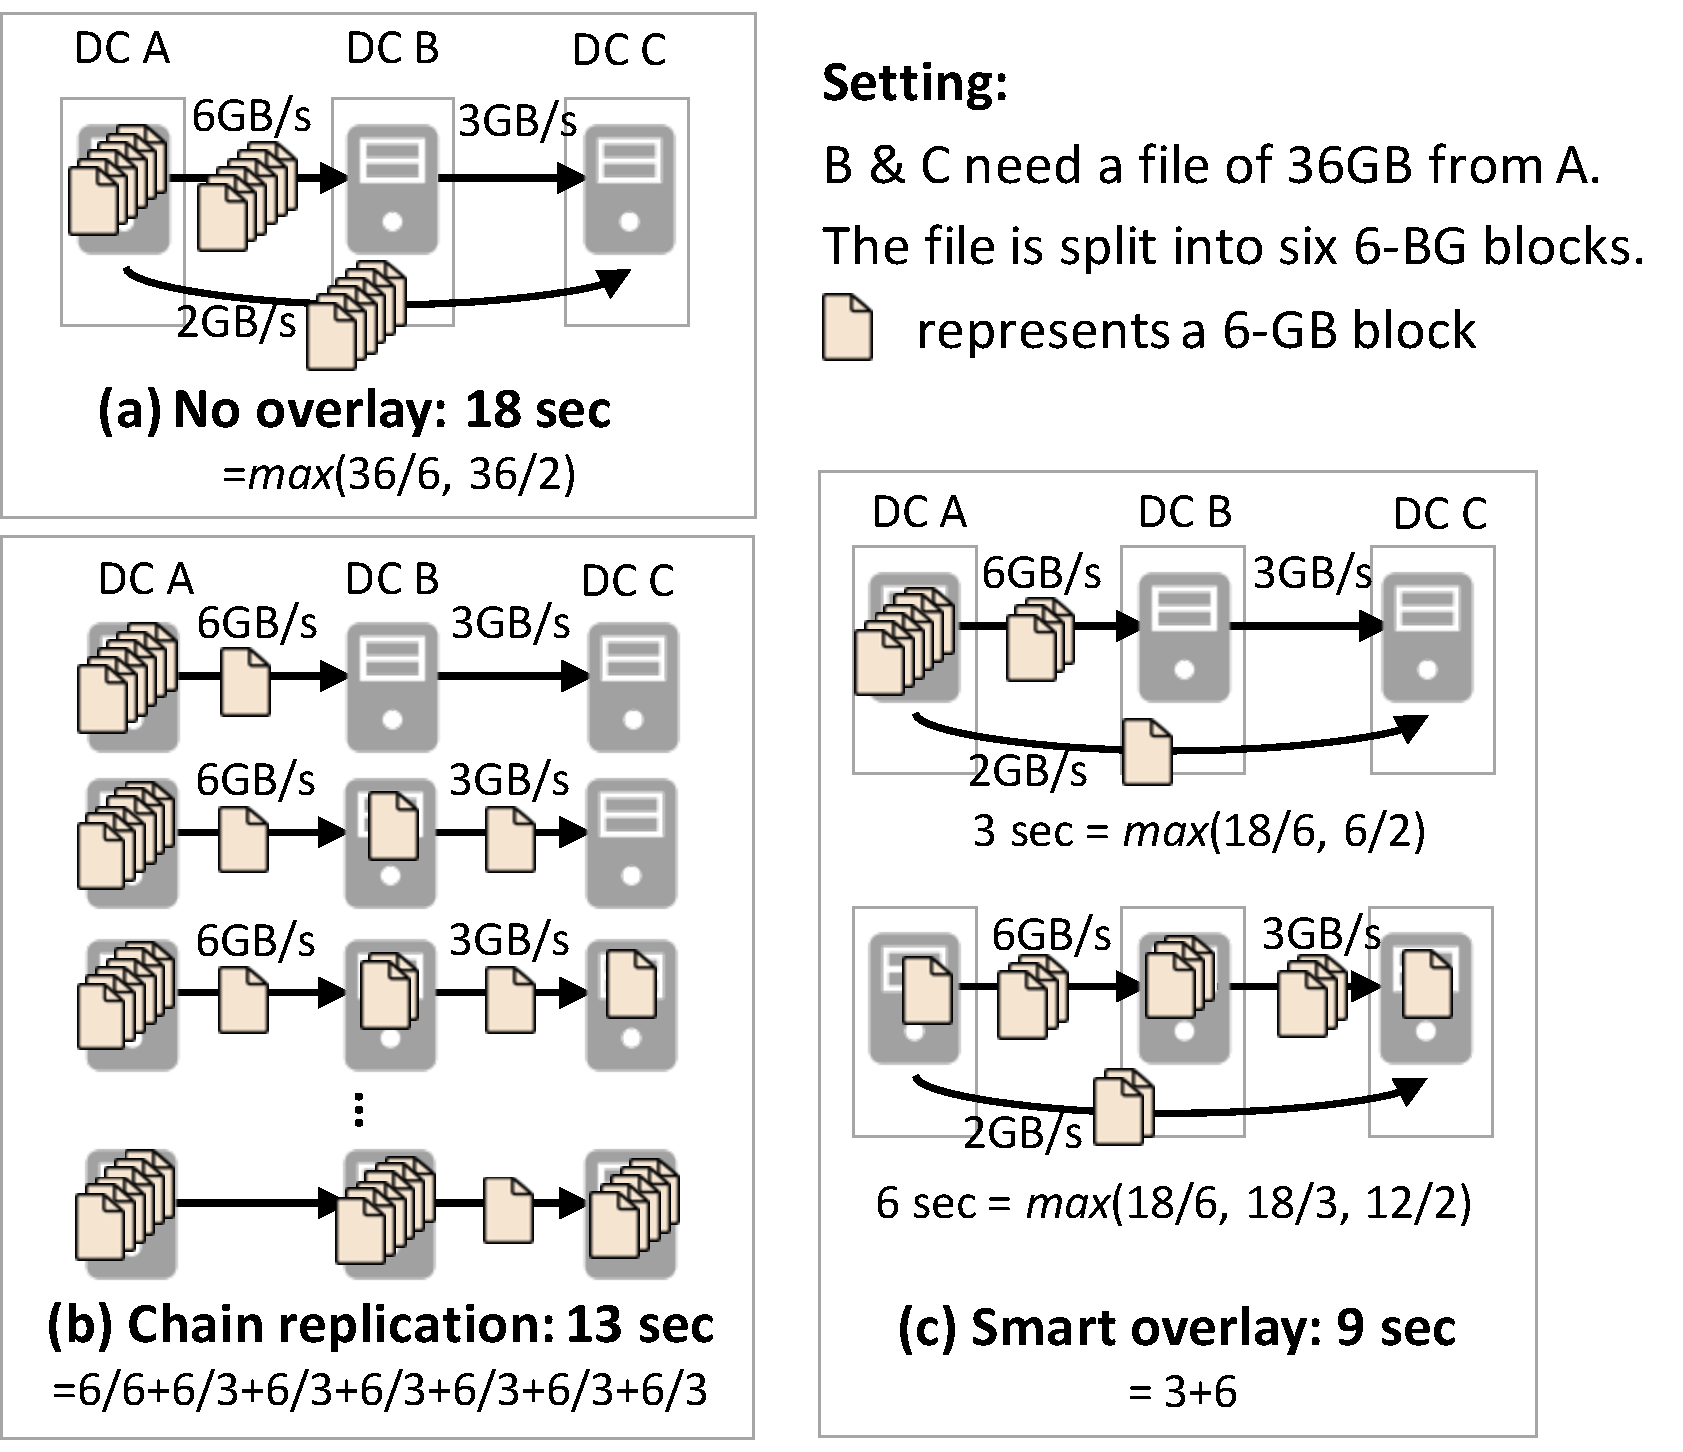
\includegraphics[width=84mm]{images/example-junchen.pdf}
\vspace{-0.4cm}
\tightcaption{An illustrative example showing the performance benefit of an application-level overlay network on inter-DC multicast.}
\label{fig:case:example}
\vspace{-0.4cm}
\end{figure}

It is known that multicast can
benefit from application-level overlays~\cite{chu2000case}.
Here we show that inter-DC multicast
completion time (defined as the duration of data transfers
until each destination DC has a full copy of the data)
can be much improved by an
application-level overlay network.\myfootnote{An application-level overlay is complementary to
prior work that focused on optimizing WAN.}

The basic idea of application-level overlay networks is
to leverage {\em bottleneck-disjoint} overlay paths.
%, which do not have common bottleneck links~\cite{datta19951}.
In the context of inter-DC overlays, two
overlay paths either traverse different sequences of DCs ({\em Type I}), or
traverse the same DCs but different sequences of
servers ({\em Type II}).
Next, we use examples to show that bottleneck-disjoint overlay paths can rise in both types, and it can be used to improve inter-DC multicast performance.

\mypara{Examples of bottleneck-disjoint overlay paths}
Recall that Figure~\ref{fig:intro} illustrates the benefits of
using Type I bottleneck-disjoint overlay paths
(i.e., going through different sequences of DCs),
$A$$\rightarrow$$B$$\rightarrow$$C$ and
$A$$\rightarrow$$C$$\rightarrow$$B$.
%Here, we examine how bottleneck-disjoint overlay paths
%in the latter
%case (i.e., same sequence of DCs but different servers) can
%be used to improve inter-DC multicast performance, and how
%prevalent they are in reality.
%Note if two paths of the same sequence of DCs are disjoint,
%at least one of them must not be bottlenecked WANs
%(because they traverse the same sequence of WAN paths).
Figure~\ref{fig:case:example} shows an example
of Type II bottleneck-disjoint overlay paths
(traversing the same sequence of DCs but different servers).
Suppose we need to replicate 36GB data from DC $A$
to $B$ and $C$ via two bottleneck-disjoint paths:
(1) $A$$\rightarrow$$C$:
from $A$ through $B$ to $C$ using IP-layer WAN routing with
2GB/s capacity, or
(2) $A$$\rightarrow$$b$$\rightarrow$$C$: from $A$ to a server
$b$ in $B$ with
6GB/s capacity and $b$ to $C$ with 3GB/s capacity.
%<<<<<<< HEAD
%Topologically, $A$ is directly connected with $B$ by a 2GB/s
%link, and
Assume the data is split into 6 6GB-blocks.
We consider three strategies.
(1) {\em Direct replication}:
if $A$ sends data directly to $B$ and $C$ via WAN paths
(Figure~\ref{fig:case:example}(b)),
the completion time is 18 seconds.
(2) {\em Simple chain replication}:
a naive use of application-level overlay paths
%=======
%Topologically, $A$ is directly connected to $B$, and
%$A$ has two paths to reach $C$: the WAN path
%which has 2GB/s capacity
%(note that this path could go through $B$), or the overlay path
%from $A$ to a server $X$ in $B$ with 6BG/s capacity,
%and then from $X$ to $C$ with 3GB/s capacity.
%To begin with, if $A$ sends the data directly to $B$ and $C$,
%as in Figure~\ref{fig:case:example}(a),
%i.e., no application-level overlay,
%the the completion time would be 18 seconds.
%If we use overlay routing but only with a simple DC-level chain
%>>>>>>> 09029e454f71e5a5e01f13f554477705e665f4ec
is to send blocks through server $b$ acting as a
store-and-relay point
(Figure~\ref{fig:case:example}(c)),
and the completion time is 13 seconds (27\% less than without overlay).
(3) {\em Optimal multicast overlay}:
Figure~\ref{fig:case:example}(d) further improves the performance by
selectively sending blocks along the two paths simultaneously,
which completes in 9 seconds (30\% less than chain replication,
and 50\% less than direct replication).


%In other words, such optimization can be achieved on the base
%of existing solutions, with no conflicts while further
%reducing the completion time.
%\jc{need to stress that multicast overlay is orthogonal to
%prior work's focus of WAN optimization}




%Fig. \ref{fig:case:example} shows three cases under different transmission strategies. Assume there are 6 DCs in the network: source DC \emph{S}, 2 intermediate DCs \emph{X} and \emph{Y}, 4 destination DCs $d_1,d_2,d_3,d_4$, and the bandwidth of both upload and download links are all 2Gbps. There is a 5G data file in the source DC \emph{S} that should be multicasted to all the 4 destination DCs. The data file is split into 5 blocks ($b_1,b_2,b_3,b_4,b_5$) each with 1G-size. (a) Directly sending data to each destination DC. The four source and destination pairs (s,d) share the link bandwidth fairly, and each is allocated to 0.5Gbps. Thus, the overall completion time in $d_i$ is 10t. (b) Build a multicast tree with chain replications on the intermediate DCs. Take $d_1$ as an example, his parent DC \emph{X} could begins to send $b_1$ with 1Gbps at the beginning of 2nd time slot because \emph{X} has already duplicated $b_1$ after 1t. So that the completion time can be reduced to 6t. (c) An optimal solution on multicast overlay network. \emph{S} sends different blocks to \emph{X} and \emph{Y} in the 1st time slot to make them share those block mutually in the next slot. Thus, in the end of 2nd slot, both \emph{X} and \emph{Y} have 3 blocks. Similarly, $d_1$ and $d_2$ are also able to share complementary blocks while download the other blocks from parent DC simultaneously. The completion time can then be further reduced to 4.5t.

\begin{figure}[t]
\centering
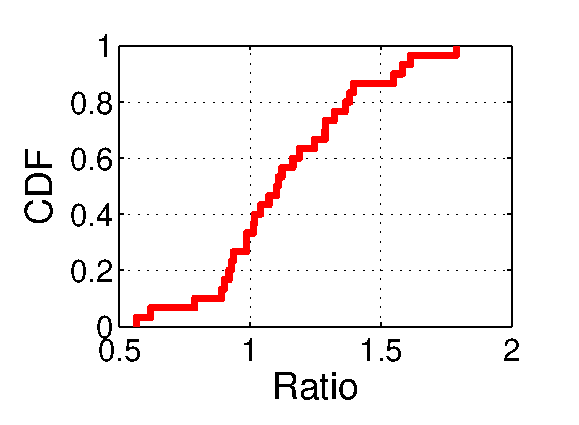
\includegraphics[width=1.5in]{images/potential_v2.eps}%DrawUp.m
\tightcaption{Even among inter-DC paths of the same DC sequence,
there is significant performance variance.
The figure shows the ratio between the available bandwidth
from $A$ to $C$ through WAN ($BW_{A\rightarrow C}$) and
that from $A$ to $C$ through $b$
($BW_{A\rightarrow b\rightarrow C}$),
across all possible $b$.}
%\jc{drop (a). avoid using notions in figure captions. captions should be standalone}\jc{please use notations in consistent with those in the text}
\label{fig:case:size}
\vspace{-0.4cm}
\end{figure}

\mypara{Bottleneck-disjoint overlay paths in the wild}
It is hard to identify all bottleneck-disjoint overlay paths,
since the dataset only has end-to-end throughput between
servers.
Instead, we show empirically that given two overlay
paths $A$$\rightarrow$$b$$\rightarrow$$C$ and $A$$\rightarrow$$C$,
where the WAN routing from DC $A$ to DC $C$ goes through DC $B$,
and $b$ is a server in $B$, they are likely to be
bottleneck-disjoint.
(These two paths are topologically identical to
Figure~\ref{fig:case:example}.)
Note if two overlay paths have different end-to-end bandwidth
(i.e., $\frac{BW_{A\rightarrow C}}{BW_{A\rightarrow b\rightarrow C}}\neq1$)
at the same time,
they should be bottleneck-disjoint.
The reason we examine such overlay path pair is that
if these pairs are widely available, we can
create a new bottleneck-disjoint path by using any server $b$
as an overlay point.
Figure~\ref{fig:case:size} shows the distribution of
$\frac{BW_{A\rightarrow C}}{BW_{A\rightarrow b\rightarrow C}}$
among all possible values of $A$, $b$, and $C$ in the dataset.
We can see that $\frac{BW_{A\rightarrow C}}{BW_{A\rightarrow b\rightarrow C}}$ is
below 0.8 or over 1.3 for about 30\% overlay pairs.
%\jc{these measurements were collected at the same time? could this variance be simply noise?} Yes, they were collected at the same time. Just as the network monitor does.



%The examples of Figure~\ref{fig:case:example} and~\ref{fig:intro}
%show that the benefits of application-level overlay networks depend
%critically on if there exist {\em disjoint} paths between
%two DCs; e.g.,
%$A$$\rightarrow$$B$$\rightarrow$$C$ and
%$A\rightarrow$$C$$\rightarrow$$B$ in Figure~\ref{fig:case:example}, and
%$A$$\rightarrow$$B$$\rightarrow$$C$ and
%$A\rightarrow$$C$$\rightarrow$$B$ in Figure~\ref{fig:intro}.
%Global-scale online service providers which have many geo-distributed
%DCs, such as \company, have disjoint paths in abundance,
%both at DC-level (e.g., consider B4~\cite{jain2013b4}'s WAN topology)
%and at server-level (e.g., in Figure~\ref{fig:case:example},
%depending on the intermediate server $b$ in $B$,
%$A$ has many overlay paths to $C$).
%A crucial question, however, is that while two overlay paths are
%physically disjoint, they might share the same bottleneck, and
%thus should be counted as not disjoint in our context.
%When two overlay paths go through different sequence of DCs,
%they are unlikely to share bottleneck.
%But when two overlay paths go through different servers but traverse
%the inter-DC WAN path, they would tend to have the same network
%bottlenecks, as WAN capacity is usually believed to be more
%limited than intra-DC networks.

%However, as shown in Figure \ref{fig:case:size},
%our empirical measurement in \company's networks shows
%otherwise.
%We consider three DCs from \company's WAN that have the same
%connectivity as in Figure~\ref{fig:case:example},
%and show the distribution of
%$\frac{BW_{A\rightarrow C}}{BW_{A\rightarrow b\rightarrow C}}$,
%the ratio between the available bandwidth
%from $A$ to $C$ through WAN ($BW_{A\rightarrow C}$) and
%that from $A$ to $C$ through $b$
%($BW_{A\rightarrow b\rightarrow C}$),
%across all possible choices of $b$.
%If WAN is indeed the bandwidth bottleneck, we should see
%$\frac{BW_{A\rightarrow C}}{BW_{A\rightarrow b\rightarrow C}}=1$,
%but the graph shows a substantial discrepancy between
%$BW_{A\rightarrow C}$ and $BW_{A\rightarrow b\rightarrow C}$,
%indicating that the available bandwidth can be bottlenecked by
%the capacity of server $b$
%($BW_{A\rightarrow C}>BW_{A\rightarrow b\rightarrow C}$),
%or the intra-DC network in DC $B$
%($BW_{A\rightarrow C}<BW_{A\rightarrow b\rightarrow C}$).
%These observations corroborate the intuition that
%{\em many physically
%disjoint overlay paths tend not to share bottleneck}.

%=======
%\mypara{Opportunities in the wild}
%Next, we use performance measured from \company's DC servers to
%investigate whether the benefits illustrated by
%Figure~\ref{fig:case:example} can be realized in a real DC WAN.
%The example of Figure~\ref{fig:case:example}
%reveals a well-known observation that the benefits of
%application-level overlay networks depend critically on if
%there exist disjoint paths between two nodes that have diverse
%performance.
%We argue that global-scale online service providers such as Google
%and \company have such disjoint paths in abundance.
%First, the disjoint paths can emerge both
%at DC-level (e.g., consider B4~\cite{b4}'s WAN topology) and
%at server-level (e.g., consider Figure~\ref{fig:case:example}
%where depending on the intermediate server in $B$,
%$A$ has many overlay paths to $C$, all via the same DC-level
%path).
%Next, we use Figure~\ref{fig:case:size} show that these paths
%have substantially diverse performance.
%We consider three DCs from \company's WAN that have the same
%connectivity as in Figure~\ref{fig:case:example}.
%We randomly selected
%>>>>>>> 09029e454f71e5a5e01f13f554477705e665f4ec


%Consider the abstract topology of \company's real network, we can also find the situations similar to the above example. There are several DC groups divided by geographical locations, and every two groups are connected through one fiber link with high bandwidth. Within each DC group, there are dozens of DCs, and in each DC, there are normally 10,000 servers. Thus, there are numbers of possible disjoint paths between any DC pairs.

%To intuitively show the benefit from disjoint paths, we make the follow measurements on the available bandwidth among three DC groups \emph{X, Y, B}. The topology is shown in Fig. \ref{fig:case:size}(a). $x_i,y_i$ and $b_i$ are servers in \emph{X, Y, B}, while any server in \emph{X} needs to go through \emph{Y} to get to any arbitrary server $b$ in \emph{B}. Let $bw(XYB)$, $bw(YB)$ denote the bandwidth between $x_i$ and $b_k$, and between $y_j$ and $b_k$, respectively, we show the fraction of $bw(XYB)$ and $bw(YB)$ in Fig. \ref{fig:case:size}(b). This figure illustrates that only in a few case (about 20\%), the available bandwidth between \emph{Y} and \emph{B} is higher than that between \emph{X} and \emph{B}, while in the majority of cases, $\frac{bw(XYB)}{bw(YB)}>1$, meaning selecting senders is not straightforward, and we do need to consider large decision spaces.

%\begin{itemize}
%
%\item Give an illustrative toy example to compare (1) directly sending data to each destination DC, (2) use chain replication, i.e., build a multicast tree with each DC being a node, (3) an optimal solution.
%{\em\bf This example is critical!}
%
%\item Briefly explain the basics of Baidu's inter-DC WAN: topology, \# of servers per DC, some estimates on how many disjoint paths are available between two DCs.
%{\em The point is that each DC has multiple disjoint paths to fetch data, despite a seemingly tree-like topology.}
%
%\item Show a CDF of $\frac{X_i\rightarrow B}{Y_i\rightarrow B}$, where $X_i\rightarrow B$, $Y_j\rightarrow B$ are the bandwidth between some server in $X$ and $B$, and between some server in $Y$ and $B$, respectively. Assume $X$ needs to go through $Y$ to get to $B$.
%{\em The point is that in a substantial fraction of cases, $\frac{X_i\rightarrow B}{Y_i\rightarrow B}>1$, meaning selecting the sender is not straightforward, we do need to consider large decision space.}
%
%\end{itemize}

\subsection{Limitations of existing solutions}
\label{subsec:motivation:baseline}

While inter-DC multicast can benefit from application-level overlay networks,
realizing these benefits in practice
is not easy. At a first glance, we can simply borrow existing techniques
from multicast overlay networks in other contexts.
But the operational experience of \company indicates
two limitations of this approach.
%However, drawing on \company's experience of
%deploying and evolving
%its multicast overlay network, we found two limitations
%of this approach.

\mypara{Existing solutions of \company}
To meet the need of rapid growth of inter-DC data replication,
\company has deployed an application-level
overlay network a few years ago.
Despite years of refinement, the overlay network
is still based on a receiver-driven decentralized
overlay multicast protocol, which
resembles what was used in other overlay networks
(such as CDNs and overlay-based live video
streaming~\cite{Andreev2013Designing,sripanidkulchai2004analysis,zhang2005coolstreaming}).
%Since then \company has refined and improved the performance of
%this solution, but the basic workflow of
%data requests remains the same.
When multiple DCs send the request of a data file
to the source DC, the requested data would flow back
through multiple stages of
intermediate servers, where the selection of senders in each stage
is driven by the receivers of the next stage in a decentralized
fashion.
%This basic workflow resembles many state-of-the-arts overlay
%protocols designed for large-scale live video
%streaming~\cite{Andreev2013Designing,sripanidkulchai2004analysis,zhang2005coolstreaming}.
%For the intermediate DCs, there is a customized store-and-forward strategy that decides whether to store the data or not and when to delete the data.
%The being used protocol in \company is a receiver-driven decentralized protocol. Once a receiver wants to download a data file, it announces the requirement to the source DC, then the required data will be forwarded to it through both the source DC and intermediate DCs. For the intermediate DCs, there is a customized store-and-forward strategy that decides whether to store the data or not and when to delete the data.
%This solution has been running for more than five years and has been continuously improved over time.
%At the same time, there are also some other solutions.
%For example, layered structures of DCs \cite{??} could simplify
%he scheduling and routing algorithm in the latency-sensitive systems
%but cannot explore more potential spaces and thus far from being
%optimal.
%Some pair-wise solutions like \cite{b4,bwe} improving inter-DC
%scheduling and routing are also not sufficient in the multicast
%overlay networks, due to the ignorance of multiple overlay paths.

%\mypara{Key limitations}
%To sum up, we can get two key lessons from the current baseline solutions.

%As data sizes continue to explode and more DCs are deployed, this protocol has begun to show two limitations.


%\begin{figure}[t]
%        \centering
%        \begin{subfigure}[b]{0.23\textwidth}
%                \centering
%                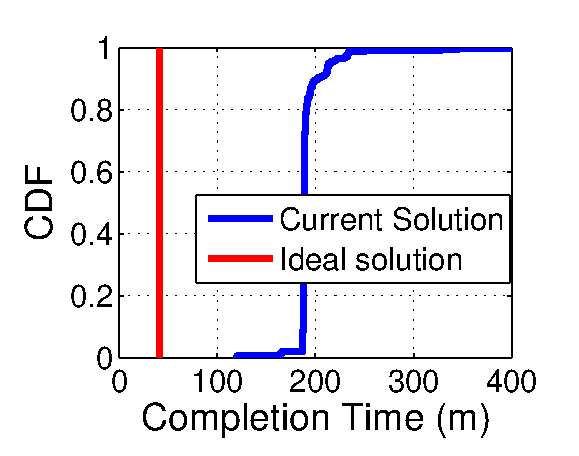
\includegraphics[width=\textwidth]{images/SEvsIdeal.eps}
%                \caption{The completion time of the 643 servers.}
%                \label{fig:motivation:observation1}
%        \end{subfigure}
%        \begin{subfigure}[b]{0.23\textwidth}
%                \centering
%                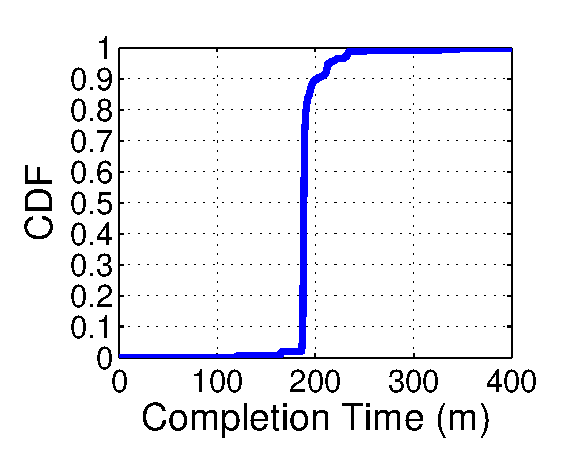
\includegraphics[width=\textwidth]{images/SE_3_cdf.eps}
%                \caption{The CDF of transmission completion time.}
%                \label{fig:motivation:observation2}
%        \end{subfigure}
%        \caption{The completion time under the current baseline solution. \jc{drop (b). add a line of 41minutes to (a). }}
%        \label{fig:motivation}
%\vspace{-0.4cm}
%\end{figure}

%\begin{itemize}
%\item Briefly describe how \company does multicast today: how to data is forwarded through an intermediate DC? what's the protocol (a receiver-driven decentralized protocol)?
%We should also stress that this solution has been running for \fillme years and has been continuously improved over time.
%
%\item Briefly mention other solutions (layered structure, hybrid approach, and why not optimizing pair-wise DC link is not sufficient)

%\jc{overall, these limitations need a bit elevation, and need to tie
%to the existing decentralized design}

%\jc{please define the flow completion time of multicast traffic first}

\noindent{\bf Limitation 1:
Inefficient local adaptation.}
The existing decentralized protocol lacks the global view and thus cannot make the optimal scheduling.
To show this, we sent a 30GB file from one DC to two destination
DCs in \company's network.
Each DC had 640 servers, each with 20Mbps upload and download
bandwidth. This 30GB file was evenly stored in all these
640 servers.
Ideally, if servers select
the best source for all blocks, the ideal
completion time will be
$\frac{30\times 1024}{640\times 20Mbps \times 60s/min} = 41$
minutes. But as shown in Figure~\ref{fig:motivation},
servers in the destination DCs on average receive data in
195 minutes (4.75 times of the optimal completion
time), and 5\% of them even take over 250 minutes.
%There are two reasons that contributed to the suboptimal
%completion time:
%1.
The key reason is that
individual servers only see from a subset of possible data sources
(servers who have already downloaded part of a file)
and thus cannot leverage all available overlay path to
maximize the throughput.
Such suboptimal performance
could occur even if the overlay
network is partially decentralized and each server does have a
global view (e.g.,~\cite{Huang2014A}),
since each server still makes local adaptations which creates potential
hotspots and congestion on overlay paths.
%2. Decisions are made based on local information and thus will be
%local optimal, such decisions possibly lead to suboptimal results
%when taken as a whole.


\begin{figure}[t]
  \centering
  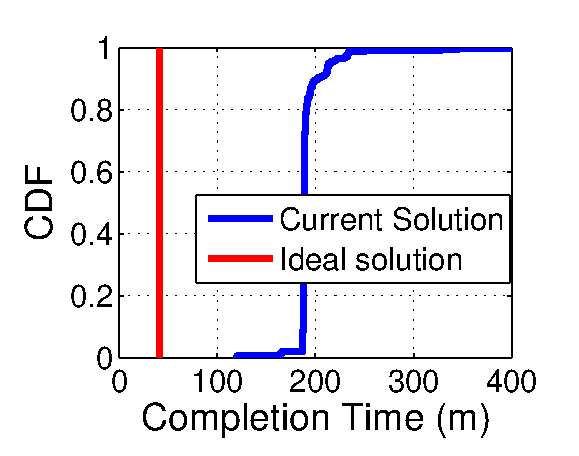
\includegraphics[width=1.5in]{images/SEvsIdeal.eps}
  \vspace{-0.2cm}
  \tightcaption{The CDF of the actual flow completion time at different servers in the destination DCs,
compared with that of the ideal solution. }
  \label{fig:motivation}
\vspace{-0.4cm}
\end{figure}

% So for a particular server, it  the unreasonable selection of data source (probably with limited bandwidth or poor connections). Without a global view, the existing decentralized protocol in anarchy cannot explore the whole decision space to find the most efficient data source.

%run an experiment in \company's DCs under a simple topology using
%real traffic trace and present the completion time.
%There is 1 source DC and 2 destination DCs
%(there are 640 servers in each DC), and the data need to be transferred is 30GB, with 20Mbps upload and download
%bandwidth on each server.
%Theoretically, the optimal overlay solution could always select
%the better source for any block of the data file, and the ideal
%completion time for destination DCs is
%$\frac{30\times 1024}{640\times 20Mbps \times 60s/min} = 41$
%minutes.
%Figure~\ref{fig:motivation} shows the results under the existing
%protocol. We see that the average completion time is about
%195 minutes, 4.75$\times$ longer than the optimal completion time.
%What's worse, it also exhibits heavy tail latency and there are
%about 5\% servers whose completion time is more than $200min$. Without global information, such inefficiency of %decentralized solution is due to two reasons: 1. Servers can't see all possible sources and can only choose from partial sources, making it not possible to explore the whole decision space to find the most efficient data source. 2. Decisions are made based on local information and thus will be local optimal, such decisions possibly lead to suboptimal results when taken as a whole.% So for a particular server, it  the unreasonable selection of data source (probably with limited bandwidth or poor connections). Without a global view, the existing decentralized protocol in anarchy cannot explore the whole decision space to find the most efficient data source.

%\jc{please explain in more details why lacking a global view will lead to so large a gap to optimal performance? is it that a server doesn't see all possible sources? is it that a server couldn't probe these sources before using them?}


%\jc{this is still a toy example. we want to use real data to show these observations. how about using the previous figure to show tail latency.}

\noindent{\bf Limitation 2:
Interference with latency-sensitive traffic.}
The existing multicast overlay network shares the same inter-DC WAN
with latency-sensitive traffic.
Despite using standard QoS techniques and giving the lowest priority to
bulk data transfers, we still see frequent interference between
latency-sensitive traffic and bursty arrivals of bulk-data multicast
requests. We monitored the bandwidth utilization of an inter-DC
link in two days during which there was a bulk data transfer at 11:00 on the 2nd day lasting for 6 hours. Figure~\ref{fig:lesson2} shows the link utilization. The blue line denotes the outgoing (outbound) bandwidth and the green line denotes the ingoing (inbound) bandwidth.
From this figure, we can see that the bulk data transfer caused high link utilization and congestion due
to lack of global coordination. As a result, the latency-sensitive online traffic experienced over
30$\times$ longer delay.

%The reason is that although all the servers worked under the standard QoS requirements, the excessive bandwidth usage of the inter-DC link still cannot be prevented due to lack of global coordination.


\begin{figure}[t!]
        \center
        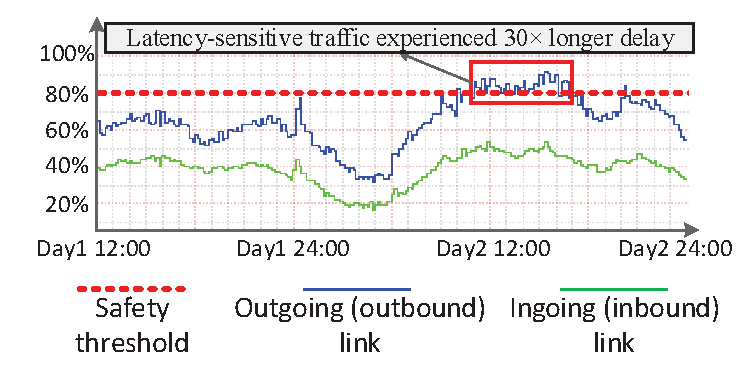
\includegraphics[width=3in]{images/nj02-M2A_0212-0216_v2.eps}
        \tightcaption{The utilization of the inter-DC link in two days. Inter-DC bulk data transfer on the 2nd day caused severe interference on latency-sensitive traffic.}
        \label{fig:lesson2}
\vspace{-0.1in}
\end{figure}

\subsection{Key observations}
The key observations from this section are:
\begin{packeditemize}
\item {\em Inter-DC multicasts} amount to a
great fraction of inter-DC traffic,
have a great variability in source-destination, and typically last for at
least tens of seconds.
\item {\em Bottleneck-disjoint overlay paths} are widely available
between geo-distributed DCs.
\item Existing solutions that use local adaptation
can have {\em suboptimal performance} and {\em negative impact on
online traffic}, due to lack of a global view and coordination.
\end{packeditemize}

%\jc{can you say something like: such inefficiency is due to the inability
%to prevent exceeding bandwidth usage by bulk-data transfers in a
%decentralized manner}
%(1) Use a figure to show that bulk data transfer can cause significant delay on latency-sensitive traffic, and (2) put some concrete numbers to show such delay can cause significant revenue loss.

%\jc{can we show some numbers on how much delay on latency-sensitive traffic during that incident? and how much losses did it cause (either in terms of application quality or in \$\$)?}

%\end{itemize}

